% ═══════════════════════════════════════════════════════════════════════════════
% INTRODUCCIÓN - INSTITUTO ATENEO DE COLIMA
% Estudio Documental: Corrupción en México (2006-2012)
% ═══════════════════════════════════════════════════════════════════════════════

\nota{
  Este capítulo introduce el problema de investigación desde una perspectiva 
  documental basada en evidencia oficial (ASF, SCJN, CNDH, CIDH, DOJ) y doctrina 
  académica arbitrada (Casar y Cejudo 2024; Merino 2024; Sandoval Ballesteros 2024).
}

\section{Contexto y perspectiva}

Con frecuencia, la historia de la corrupción en México suele narrarse al revés: la atención pública se concentra en el escándalo pasajero, la consigna viral o el enfrentamiento partidista, mientras rara vez se analiza con la cabeza fría el proceso institucional que permitió llegar a ese desenlace y el costo humano que recayó sobre la población. Así como detrás de los resultados visibles existen siempre planes, omisiones o rutinas acumuladas, el propósito de este reporte no consistió en repartir culpas por simpatía política ni en reproducir el ruido mediático, sino en examinar ---mediante evidencia oficial, auditorías y resoluciones judiciales--- qué falló estructuralmente en tres episodios decisivos y de qué manera sus secuelas comprometen lo más valioso para una sociedad: la vida, la salud, la seguridad y el patrimonio colectivo.

Desde la perspectiva científica, la corrupción constituye un fenómeno multidimensional que trasciende el plano estrictamente moral o penal para consolidarse como un problema estructural con repercusiones directas sobre el erario, la calidad de los servicios públicos, la vigencia de los derechos humanos y la legitimidad democrática \citep{inegi2016,monsivais2020,reyesheroles2003}. Su persistencia a través de distintas administraciones revela la consolidación de una corrupción sistémica y estructural, en la que las reglas formales son capturadas por redes de poder lícitas e ilícitas y la impunidad se institucionaliza \citep{casar2024,merino2024,sandoval2024}.

En este estudio se delimitó como periodo nuclear el sexenio de Felipe Calderón Hinojosa (2006--2012), administración que concluyó con una calificación de 34 sobre 100 puntos para México en el Índice de Percepción de la Corrupción (IPC) de Transparencia Internacional (2026). Durante esa etapa se gestaron expedientes de alto impacto cuyas consecuencias jurídicas, financieras y sociales se extendieron hasta noviembre de 2026, según se documentó en informes de la Auditoría Superior de la Federación (\siglas{asf}), sentencias de la Suprema Corte de Justicia de la Nación (\siglas{scjn}), recomendaciones de la Comisión Nacional de los Derechos Humanos (\siglas{cndh}), informes de la Comisión Interamericana de Derechos Humanos (\siglas{cidh}) y procesos penales y civiles sustanciados en tribunales de Estados Unidos \citep{asf2013,asf2015,asf2016,cidh2020,cndh2009,doj2024,scjn2010,scjn2025,uif2025,uif2026}.

La investigación examinó tres casos principales representativos de mecanismos diferenciados: la captura del aparato de seguridad pública y el desvío contractual en el caso de Genaro García Luna; las deficiencias de preinversión y los pasivos transexenales en la Refinería Bicentenario en Tula, Hidalgo; y la subrogación desregulada con conflicto de interés en la Guardería ABC. De manera complementaria, se incorporaron dos casos de contraste contemporáneo (el saqueo hospitalario en Veracruz y la Refinería Olmeca en Dos Bocas) con el fin exclusivo de contrastar el impacto verificable sobre las víctimas frente al sesgo del encuadre mediático (framing). El informe se organizó conforme a los estándares metodológicos de Hernández Sampieri, Fernández Collado y Baptista Lucio (2014), integrando justificación, planteamiento, marco teórico fortalecido con doctrina mexicana, diseño mixto DIAC, análisis de casos, discusión de rigor y limitaciones, conclusiones, referencias y apéndices instrumentales.

\section{Objetivos del estudio}

Este estudio documental se propuso tres objetivos centrales:

\begin{itemize}
  \item Analizar los mecanismos causales y los efectos estructurales ---institucionales, financieros y en materia de derechos humanos--- de la corrupción en México durante el sexenio 2006--2012 mediante un diseño mixto de modelo dominante cualitativo (DIAC: CUAL + cuan).
  
  \item Documentar, mediante evidencia oficial verificable, cómo decisiones administrativas adoptadas hace más de una década continuaron generando pasivos fiscales, litigios y demandas de justicia vigentes en 2026.
  
  \item Contrastar el daño real acreditado en auditorías y resoluciones judiciales con las narrativas mediáticas (framing) que suelen simplificar fenómenos complejos en consignas virales.
\end{itemize}

% FIGURA PENDIENTE
\begin{figure}[H]
\centering
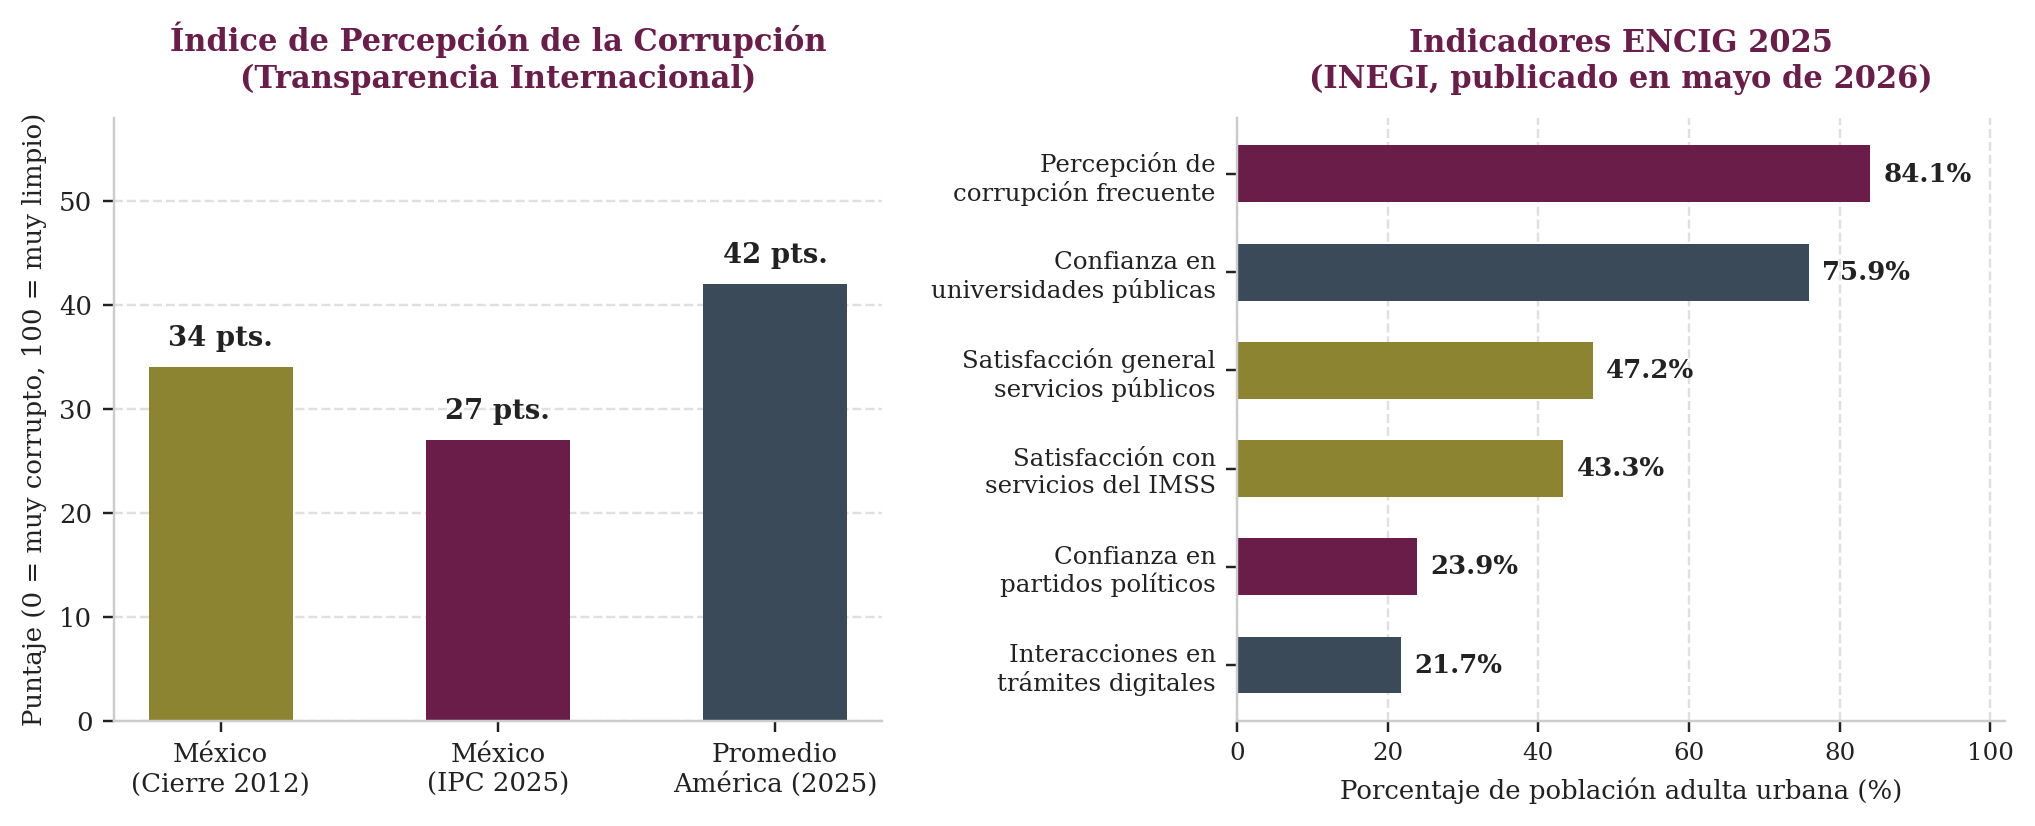
\includegraphics[width=0.9\textwidth]{img/image3.png} % Figura 1: Evolución IPC 2012 vs 2025 + ENCIG 2025
\caption{Evolución del Índice de Percepción de la Corrupción (2012 vs. 2025) e indicadores nacionales de la ENCIG 2025. Fuente: Elaboración propia con datos de Transparencia Internacional (2026) e INEGI (2026).}
\label{fig:ipc-encig}
\end{figure}